\documentclass[11pt]{article}
\usepackage{amsmath,amssymb,amsthm}
\usepackage{graphicx}
\usepackage{hyperref}

\newtheorem{claim}{Claim}

\title{Disproof of the Archimedean Property from Field and Order Axioms}
\author{LU Chen Yu}
\date{\today}

\begin{document}
\maketitle

\begin{claim}
\label{clm:target}
The Archimedean property can be proved from only the Field Axioms and Order Axioms.
\end{claim}

\paragraph{Archimedean Property}
For an ordered field $F$, the Archimedean property states:
\[
\forall x \in F,\ \exists n \in \mathbb{N}\text{ such that }n>x.
\]

\paragraph{Completeness Axiom}
Every nonempty subset $S\subseteq\mathbb{R}$ that is bounded above has a least upper bound in $\mathbb{R}$.

\begin{figure}[h]
\centering
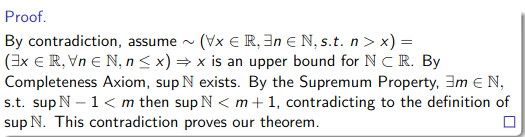
\includegraphics[width=0.8\textwidth]{images/figure_1.png}
\caption{Proof sketch using Completeness Axiom}
\end{figure}



\paragraph{Counterexample setup.}
Define a non-Archimedean ordered field $\mathbb{F}$ with the required assumptions:
\begin{itemize}
    \item Assumption 1: $\mathbb{F}$ = $\{\frac{p(x)}{q(x)}: p(x), q(x) \in \mathbb{Z}[x], q(x) \neq 0\}$.
	\item Assumption 2: $\mathbb{F}$ is ordered by $\frac{p(x)}{q(x)} > 0$ if the leading coefficient of $p(x)$ and $q(x)$ are both positive or both negative.
\end{itemize}

\paragraph{Verification of assumptions.}
We verify that $\mathbb{F}$ satisfies both field axioms and order axioms.

\textbf{Field axioms.}
Write $\mathbb{F}=\mathrm{Frac}(\mathbb{Z}[x])$. Since $\mathbb{Z}[x]$ is an integral domain, its fraction field exists.
For $a=\frac{p}{q}$, $b=\frac{r}{s}$ (with $q,s\neq 0$), define
\[
a+b=\frac{ps+rq}{qs},\qquad ab=\frac{pr}{qs}.
\]
Then $a+b,ab\in\mathbb{F}$ (closure). The additive identity is $0=\frac{0}{1}$, multiplicative identity is $1=\frac{1}{1}$,
\[
-a=\frac{-p}{q},\qquad a^{-1}=\frac{q}{p}\ \text{for }a\neq 0.
\]
Associativity, commutativity, and distributivity are inherited from polynomial arithmetic, so all field axioms hold.

\textbf{Order axioms.}
Define positivity by eventual sign (equivalently by sign of leading term):
\[
\frac{p(x)}{q(x)}>0
\iff
\text{for all sufficiently large }x,\ p(x)q(x)>0.
\]
This is well-defined on fractions and gives trichotomy: for every $a\in\mathbb{F}$, exactly one of $a>0$, $a=0$, $-a>0$ holds.
Also,
\[
a>0,\ b>0\implies a+b>0,\ ab>0,
\]
because eventually positive functions stay positive under addition and multiplication. Hence the order is compatible with field operations, so $\mathbb{F}$ is an ordered field.

\paragraph{Failure of conclusion.}
Let $t=\frac{x}{1}\in\mathbb{F}$. For any $n\in\mathbb{N}$,
\[
t-n=\frac{x-n}{1}>0
\]
because $x-n$ has positive leading coefficient, so it is positive for sufficiently large $x$.
Thus $t>n$ for every $n\in\mathbb{N}$. Therefore no natural number exceeds $t$, so the Archimedean property fails in $\mathbb{F}$.

\paragraph{Conclusion.}
Therefore, Claim~\ref{clm:target} is false.

\end{document}
